%%%%%%%%%%%%%%%%%%%%%%%%%%%%%%%%%%%%%%%%%%%%%%%%%%%%%%%%%%%%%%%%%%%%%%%%%%%%%%%%
%% Plantilla de memoria en LaTeX para la ETSIT - Universidad Rey Juan Carlos
%%
%% Por Gregorio Robles <grex arroba gsyc.urjc.es>
%%     Grupo de Sistemas y Comunicaciones
%%     Escuela Técnica Superior de Ingenieros de Telecomunicaci�n
%%     Universidad Rey Juan Carlos
%% (muchas ideas tomadas de Internet, colegas del GSyC, antiguos alumnos...
%%  etc. Muchas gracias a todos)
%%
%% La última versión de esta plantilla est� siempre disponible en:
%%     https://github.com/gregoriorobles/plantilla-memoria
%%
%% Para obtener PDF, ejecuta en la shell:
%%   make
%% (las imágenes deben ir en PNG o JPG)

%%%%%%%%%%%%%%%%%%%%%%%%%%%%%%%%%%%%%%%%%%%%%%%%%%%%%%%%%%%%%%%%%%%%%%%%%%%%%%%%

\documentclass[a4paper, spanish, 12pt]{book}
%\usepackage[T1]{fontenc}

\usepackage[a4paper, left=2.5cm, right=2.5cm, top=3cm, bottom=3cm]{geometry}
\usepackage{times}
\usepackage[latin1]{inputenc}
\usepackage[spanish]{babel} % Comenta esta l�nea si tu memoria es en ingl�s
\usepackage{url}
%\usepackage[dvipdfm]{graphicx}
\usepackage{graphicx}
\usepackage{float}  %% H para posicionar figuras
\usepackage[nottoc, notlot, notlof, notindex]{tocbibind} %% Opciones de �ndice
\usepackage{latexsym}  %% Logo LaTeX
\usepackage{titlesec}
\setcounter{secnumdepth}{4}

\title{Memoria del Proyecto}
\author{Nombre del autor}

\renewcommand{\baselinestretch}{1.5}  %% Interlineado

\begin{document}

\renewcommand{\refname}{Bibliograf\'ia}  %% Renombrando
\renewcommand{\appendixname}{Ap\'endice}

\makeatletter
% we use \prefix@<level> only if it is defined
\renewcommand{\@seccntformat}[1]{%
  \ifcsname prefix@#1\endcsname
    \csname prefix@#1\endcsname
  \else
    \csname the#1\endcsname\quad
  \fi}
% define \prefix@section
\newcommand\prefix@subsubsection{\thesubsubsection}
\makeatother

%%%%%%%%%%%%%%%%%%%%%%%%%%%%%%%%%%%%%%%%%%%%%%%%%%%%%%%%%%%%%%%%%%%%%%%%%%%%%%%%
% PORTADA

\begin{titlepage}
\begin{center}
\begin{tabular}[c]{c c}
%\includegraphics[bb=0 0 194 352, scale=0.25]{logo} &
\includegraphics[scale=0.25]{img/logo_vect.png} &
\begin{tabular}[b]{l}
\Huge
\textsf{UNIVERSIDAD} \\
\Huge
\textsf{REY JUAN CARLOS} \\
\end{tabular}
\\
\end{tabular}

\vspace{3cm}

\Large
Grado en Tecnolog\'ias de las Telecomunicaciones

\vspace{0.4cm}

\large
Curso Acad\'emico 2015/2016

\vspace{0.8cm}

Trabajo Fin de Grado

\vspace{2.5cm}

\LARGE
An\'alisis de proyectos FOSS

\vspace{4cm}

\large
Autor : Joel Peralta Rodr\'iguez \\
Tutor : Dr. Gregorio Robles
\end{center}
\end{titlepage}

\newpage
\mbox{}
\thispagestyle{empty} % para que no se numere esta pagina


%%%%%%%%%%%%%%%%%%%%%%%%%%%%%%%%%%%%%%%%%%%%%%%%%%%%%%%%%%%%%%%%%%%%%%%%%%%%%%%%
%%%% Para firmar
\clearpage
\pagenumbering{gobble}
\chapter*{}

\vspace{-4cm}
\begin{center}
\LARGE
\textbf{Proyecto Fin de Carrera}

\vspace{1cm}
\large
An\'alisis de proyectos FOSS

\vspace{1cm}
\large
\textbf{Autor :} Joel Peralta Rodr\'iguez \\
\textbf{Tutor :} Dr. Gregorio Robles Mart\'inez

\end{center}

\vspace{1cm}
La defensa del presente Proyecto Fin de Carrera se realiz\'o el d\'ia \qquad$\;\,$ de junio de 2016, siendo calificada por el siguiente tribunal:


\vspace{0.5cm}
\textbf{Presidente:}

\vspace{1.2cm}
\textbf{Secretario:}

\vspace{1.2cm}
\textbf{Vocal:}


\vspace{1.2cm}
y habiendo obtenido la siguiente calificaci\'on:

\vspace{1cm}
\textbf{Calificaci\'on:}


\vspace{1cm}
\begin{flushright}
Fuenlabrada, a \qquad$\;\,$ de junio de 2016
\end{flushright}

%%%%%%%%%%%%%%%%%%%%%%%%%%%%%%%%%%%%%%%%%%%%%%%%%%%%%%%%%%%%%%%%%%%%%%%%%%%%%%%%
%%%% Dedicatoria

\chapter*{}
\pagenumbering{Roman} % para comenzar la numeracion de paginas en numeros romanos
\begin{flushright}
\textit{Dedicado a \\
mi familia / mi abuelo / mi abuela}
\end{flushright}

%%%%%%%%%%%%%%%%%%%%%%%%%%%%%%%%%%%%%%%%%%%%%%%%%%%%%%%%%%%%%%%%%%%%%%%%%%%%%%%%
%%%% Agradecimientos

\chapter*{Agradecimientos}
%\addcontentsline{toc}{chapter}{Agradecimientos} % si queremos que aparezca en el �ndice
\markboth{AGRADECIMIENTOS}{AGRADECIMIENTOS} % encabezado

Aqu\'i vienen los agradecimientos\ldots Aunque est\'a bien acordarse de la pareja,
no hay que olvidarse de dar las gracias a tu madre, que aunque a veces no lo
parezca disfrutar\'a tanto de tus logros como t\'u\ldots Adem\'as, la pareja quiz\'as
no sea para siempre, pero tu madre s\'i.

%%%%%%%%%%%%%%%%%%%%%%%%%%%%%%%%%%%%%%%%%%%%%%%%%%%%%%%%%%%%%%%%%%%%%%%%%%%%%%%%
%%%% Resumen

\chapter*{Resumen}
%\addcontentsline{toc}{chapter}{Resumen} % si queremos que aparezca en el �ndice
\markboth{RESUMEN}{RESUMEN} % encabezado

Aqu\'i viene un resumen del proyecto. Ha de constar de tres o cuatro p\'arrafos,
donde se presente de manera clara y concisa de qu\'e va el proyecto. Han
de quedar respondidas las siguientes preguntas:

\begin{itemize}
  \item ?`De qu\'e va este proyecto? ?`Cu\'al es su objetivo principal?
  \item ?`C\'omo se ha realizado? ?`Qu\'e tecnolog\'ias est\'an involucradas?
  \item ?`En qu\'e contexto se ha realizado el proyecto? ?`Es un proyecto
dentro de un marco general?
\end{itemize}

Lo mejor es escribir el resumen al final.

%%%%%%%%%%%%%%%%%%%%%%%%%%%%%%%%%%%%%%%%%%%%%%%%%%%%%%%%%%%%%%%%%%%%%%%%%%%%%%%%
%%%% Resumen en ingl\'es

\chapter*{Summary}
%\addcontentsline{toc}{chapter}{Summary} % si queremos que aparezca en el �ndice
\markboth{SUMMARY}{SUMMARY} % encabezado

Here comes a translation of the ``Resumen'' into English. Please, double check
it for correct grammar and spelling. As it is the translation of the ``Resumen'',
which is supposed to be written at the end, this as well should be followed out
just before submitting.


%%%%%%%%%%%%%%%%%%%%%%%%%%%%%%%%%%%%%%%%%%%%%%%%%%%%%%%%%%%%%%%%%%%%%%%%%%%%%%%%
%%%%%%%%%%%%%%%%%%%%%%%%%%%%%%%%%%%%%%%%%%%%%%%%%%%%%%%%%%%%%%%%%%%%%%%%%%%%%%%%
% ÍNDICES %
%%%%%%%%%%%%%%%%%%%%%%%%%%%%%%%%%%%%%%%%%%%%%%%%%%%%%%%%%%%%%%%%%%%%%%%%%%%%%%%%

% Las buenas noticias es que los índices se generan autom�ticamente.
% Lo único que tienes que hacer es elegir cuáles quieren que se generen,
% y comentar/descomentar esa instrucción de LaTeX.

%%%% Índice de contenidos
\tableofcontents
%%%% Índice de figuras
\cleardoublepage
%\addcontentsline{toc}{chapter}{Lista de figuras} % para que aparezca en el indice de contenidos
\listoffigures % indice de figuras
%%%% Índice de tablas
%\cleardoublepage
%\addcontentsline{toc}{chapter}{Lista de tablas} % para que aparezca en el indice de contenidos
%\listoftables % indice de tablas


%%%%%%%%%%%%%%%%%%%%%%%%%%%%%%%%%%%%%%%%%%%%%%%%%%%%%%%%%%%%%%%%%%%%%%%%%%%%%%%%
%%%%%%%%%%%%%%%%%%%%%%%%%%%%%%%%%%%%%%%%%%%%%%%%%%%%%%%%%%%%%%%%%%%%%%%%%%%%%%%%
% INTRODUCCIÓN %
%%%%%%%%%%%%%%%%%%%%%%%%%%%%%%%%%%%%%%%%%%%%%%%%%%%%%%%%%%%%%%%%%%%%%%%%%%%%%%%%

\cleardoublepage
\chapter{Introducci\'on}
\label{sec:intro} % etiqueta para poder referenciar luego en el texto con~\ref{sec:intro}
\pagenumbering{arabic} % para empezar la numeración de página con números

En este proyecto se ha realizado un an\'alisis del ecosistema de proyectos de
software libre que podemos encontrar en la red, centr\'andose especialmente en
la plataforma Github. Mediante este an\'alisis se ha intentado dar a conocer las
caracter\'isticas de este entorno adem\'as de determinar las peculiaridades que
aportan los datos obtenidos a la formaci\'on y desarrollo del Free Open Source Software.

A continuaci\'on, para una mejor comprensi\'on del proyecto, se explicar\'an el
contexto del mismo, su estructura y las motivaciones personales para realizarlo.

\section{Contexto}
\label{sec:contexto}

En un sector tan amplio como el de la programaci\'on, en el cual se pueden dise\~nar
y desarrollar soluciones a problemas muy diversos, surge el planteamiento de este
proyecto fin de grado para tratar de buscar las caracter\'isticas comunes de
diferentes proyectos de software libre y de sus desarrolladores.

Con la obtenci\'on de la informaci\'on presente en estos proyectos, se pretende
realizar una comparativa de los diferentes tipos de software libre que se est\'an
desarrollando en la actualidad, adem\'as de sus caracter\'isticas en cuanto a
copyrights y licencias. De esta manera se podr\'an entender mejor las cualidades
que ha de tener un determinado software para ser libre y abierto, y para poder
progresar y obtener mayor relevancia en el mundo del Free Open Source Software.

Esta informaci\'on legal, aunque secundaria, puede suponer un punto clave para
un determinado proyecto, puesto que en la comunidad Free Open Source, un aspecto
muy importante del software debe ser su libertad de uso, acceso al c\'odigo y distribuci\'on
y modificaci\'on del mismo.

Este proceso de an\'alisis se realiza en el contexto de una aplicaci\'on
web, por tanto, el resultado del mismo podr\'a ser accesible a m\'ultiples usuarios
que busquen el tipo de proyecto que se est\'a realizando en la actualidad, o a
colaboradores activos de proyectos de software libre, o caracter\'isticas de distintos
proyectos que les permitan tomar conciencia de la importancia de que el nuevo software
que est\'an desarrollando sea libre y accesible para todo el mundo.

%\subsection{Estilo}
%\label{subsec:estilo}
%
%Sobre el uso de las comas\footnote{\url{http://narrativabreve.com
%/2015/02/opiniones-de-un-corrector-de-estilo-11-recetas-para-escribir-correctamente-la-coma.html}}
%
% \begin{figure}
%    \centering
%    \includegraphics[bb=0 0 800 600, width=12cm, keepaspectratio]{img/foro1}
%    \caption{P\'agina con enlaces a hilos}
%    \label{figura:foro_hilos}
% \end{figure}
%
%{\footnotesize
%\begin{verbatim}
%    From gaurav at gold-solutions.co.uk  Fri Jan 14 14:51:11 2005
%    From: gaurav at gold-solutions.co.uk (gaurav_gold)
%    Date: Fri Jan 14 19:25:51 2005
%    Subject: [Mailman-Users] mailman issues
%    Message-ID: <003c01c4fa40$1d99b4c0$94592252@gaurav7klgnyif>
%
%    Dear Sir/Madam,
%    How can people reply to the mailing list?  How do i turn off
%    this feature? How can i also enable a feature where if someone
%    replies the newsletter the email gets deleted?
%    Thanks
%
%    From msapiro at value.net  Fri Jan 14 19:48:51 2005
%    From: msapiro at value.net (Mark Sapiro)
%    Date: Fri Jan 14 19:49:04 2005
%    Subject: [Mailman-Users] mailman issues
%    In-Reply-To: <003c01c4fa40$1d99b4c0$94592252@gaurav7klgnyif>
%    Message-ID: <PC173020050114104851057801b04d55@msapiro>
%
%    gaurav_gold wrote:
%    >How can people reply to the mailing list?  How do i turn off
%    this feature? How can i also enable a feature where if someone
%    replies the newsletter the email gets deleted?
%
%    See the FAQ
%    >Mailman FAQ: http://www.python.org/cgi-bin/faqw-mm.py
%    article 3.11
%\end{verbatim}
%}

\section{Motivaciones personales}
\label{sec:motivaciones}

La principal motivaci\'on por la que se decidi\'o realizar este proyecto es el
proceso de an\'alisis, filtrado y representaci\'on de grandes cantidades de datos.
Adem\'as al tratarse de una aplicaci\'on web, engloba diferentes
aspectos importantes del desarrollo de software, como son el desarrollo web,
t\'ecnicas de Big Data y tambi\'en el desarrollo de soluciones a problemas de
\'indole acad\'emica.

Por otra parte, los diferentes tipos de tecnolog\'ias utilizadas para desarrollar
el proyecto, hac\'ian que este fuera m\'as interesante desde un punto de vista
educativo y de desarrollo de las habilidades program\'aticas.

\section{Estructura de la memoria}
\label{sec:estructura}

Para una mejor lectura, se desglosa a continuaci\'on la estructura de este documento:

\begin{itemize}
  \item \textbf{1. Introducci\'on.} Con el objetivo de enmarcar el proyecto en
  su contexto.

  \item \textbf{2. Objetivos.} Secci\'on en la que se muestran los objetivos
  finales y parciales del proyecto.

  \item \textbf{3. Estado del arte.} Donde se muestran las tecnolog\'ias y metodolog\'ias
  utilizadas para elaborar las distintas partes del proyecto.

  \item \textbf{4. Dise\~no e implementaci\'on.} En esta secci\'on se elabora una
  explicaci\'on del proceso realizado y el dise\~no previo de este proceso, para
  una correcta realizaci\'on del proyecto.

  \item \textbf{5. Resultados.} Para mostrar los resultados obtenidos tras la realizaci\'on
  del proyecto.

  \item \textbf{6. Conclusiones.} Donde se enumeran las conclusiones obtenidas de
  los resultados de la secci\'on anterior.

  \item \textbf{7. Ap\'endices.} Secci\'on en la que se muestra cualquier informaci\'on
  adicional para la adecuada comprensi\'on de la memoria.

  \item \textbf{8. Bibliograf\'ia.} Lista de fuentes de informaci\'on en las cuales
  se basa la este documento.
\end{itemize}



%%%%%%%%%%%%%%%%%%%%%%%%%%%%%%%%%%%%%%%%%%%%%%%%%%%%%%%%%%%%%%%%%%%%%%%%%%%%%%%%
%%%%%%%%%%%%%%%%%%%%%%%%%%%%%%%%%%%%%%%%%%%%%%%%%%%%%%%%%%%%%%%%%%%%%%%%%%%%%%%%
% OBJETIVOS %
%%%%%%%%%%%%%%%%%%%%%%%%%%%%%%%%%%%%%%%%%%%%%%%%%%%%%%%%%%%%%%%%%%%%%%%%%%%%%%%%

\cleardoublepage
\chapter{Objetivos}
\label{chap:objetivos}

\section{Objetivo general}
\label{sec:objetivo-general}

El objetivo principal del proyecto es dar una visi\'on general de distintos
proyectos de software libre que se desarrollan en la actualidad, para comprender
mejor el ecosistema Open Source y ofrecer a los posibles usuarios una manera de
encontrar proyectos populares en los que colaborar, usuarios activos que puedan
unirse a nuevos proyectos y de observar las licencias, herramientas y
lenguajes de progrmaci\'on m\'as populares entre los usuarios.

\section{Objetivos espec\'ificos}
\label{sec:objetivos-especificos}

Para llevar a cabo el objetivo principal, se han cumplido una serie de objetivos
secundarios que se describir\'an a continuaci\'on:

\begin{itemize}

\item Familiarizarse con la herramienta Scancode Toolkit que servir\'a para
analizar proyectos desde la terminal de Unix y posteriormente analizar la
infomaci\'on devuelta por dicha herramienta.

\item Inicializar el proyecto Django/Python que albergar\'a la aplicaci\'on
web en la que se engloba el an\'alisis de proyectos.

\item Adaptar la herramienta para ser usada como un m\'odulo de Python
y poder tener mayor versatilidad al analizar proyectos en distintos formatos.

\item Desarrollar una API REST cuyos recursos servir\'an para analizar proyectos
y devolver los resultados en un formato f\'acilmente representable en el navegador.

\item Crear los modelos de la base de datos y almacenar los
primeros proyectos FOSS que ser\'an posteriormente representados.

\item Montar la estructura del framework web AngularJS para realizar de manera
correcta y ordenada la representaci\'on de los datos obtenidos de la API.

\item Representar los datos obtenidos de la API REST mediante la librer\'ia
nvd3 basada en d3.js en diferentes gr\'aficos.

\item Corregir la est\'etica de la p\'agina, adem\'as de distintos problemas de
adaptaci\'on entre el back-end (Python) y el front-end (JavaScript).

\item Analizar mayor n\'umero de proyectos para obtener mayor n\'umero de datos
que ayuden a sacar conclusiones del entorno Open Source.

\end{itemize}

\section{Planificaci\'on temporal}
\label{sec:planificacion-temporal}

La planificaci\'on temporal del proyecto queda representada por el gr\'afico del
ap\'endice X para una mejor comprensi\'on de los plazos tomados para la consecuci\'on
de los distintos objetivos.

%%%%%%%%%%%%%%%%%%%%%%%%%%%%%%%%%%%%%%%%%%%%%%%%%%%%%%%%%%%%%%%%%%%%%%%%%%%%%%%%
%%%%%%%%%%%%%%%%%%%%%%%%%%%%%%%%%%%%%%%%%%%%%%%%%%%%%%%%%%%%%%%%%%%%%%%%%%%%%%%%
% ESTADO DEL ARTE %
%%%%%%%%%%%%%%%%%%%%%%%%%%%%%%%%%%%%%%%%%%%%%%%%%%%%%%%%%%%%%%%%%%%%%%%%%%%%%%%%

\cleardoublepage
\chapter{Estado del arte}

En esta secci\'on se presentar\'an las tecnolog\'ias utilizadas en el desarrollo
del proyecto, tanto en el an\'alisis de datos como en la representaci\'on de los
mismos.

Para ello se realizar\'a una descripci\'on general de cada herramienta y las
cualidades espec\'ificas por las cuales han sido utilizadas.

%Puedes citar libros, como el de Bonabeau et al. sobre procesos estigm\'argicos~\cite{bonabeau:_swarm}.
%
%Tambi\'en existe la posibilidad de poner notas al pie de p\'agina, por ejemplo,
%una para indicarte que visite la p\'agina de
%LibreSoft\footnote{\url{http://www.libresoft.es}}.

\section{Free Open Source Software (FOSS)}
\label{sec:FOSS}

Para entender el concepto de FOSS, se explican a continuaci\'on los requisitos
del software para ser libre y abierto, estos dos t\'erminos siguen las directrices
de dos organizaciones, Free Software Foundation~\cite{fsf} y
Open Source Initiative~\cite{opensource} respectivamente.

\begin{figure}[H]
  \centering
  
\includegraphics[width=7cm, keepaspectratio]{img/fsf}
\end{figure}

A continuaci\'on se especificar\'an las caracter\'isticas de cada uno de ellos.

Para que el software se considere libre, ha de cumplir estas cuatro libertades:

\begin{itemize}

\item Libertad de uso del programa por cualquier raz\'on.

\item Libertad de acceso, estudio y modifici\'on del c\'odigo.

\item Libertad de copia y distribuci\'on.

\item Libertad de mejora y publicaci\'on de las mismas.

\end{itemize}

Para las libertades 1 y 3, es necesario que el c\'odigo fuente del software sea
de libre acceso al p\'ublico.

\begin{figure}[H]
  \centering
  
\includegraphics[height=5cm, width=4cm, keepaspectratio]{img/Opensource}
\end{figure}

Por otro lado, la iniciativa Open Source se centra menos en las caracter\'isticas
\'eticas del software libre, y m\'as en las t\'ecnicas y econ\'omicas. Sin embargo,
son muy pocos los proyectos de software que siendo reconocidos por la Ola Open
Source Initiative, no sea considerado Free Software. Por esta raz\'on se suele
utilizar el t\'ermino Free Open Source Software.

\section{Python}
\label{sec:python}

Python es un lenguaje de programaci\'on multiparadigma, al permitir la programaci\'on
orientada a objetos, declarativa y funcional. Es interpretado, por no requerir
compilaci\'on, con tipado din\'amico y multiplataforma~\cite{python}.

Este lenguaje fue publicado por Guido van Rossum en 1991 en los Pa\'ises Bajos
como un proyecto de software libre. Actualmente se encuentra bajo una licencia
Python Software Foundation License, compatible con la licencia general de GNU a partir
de su versi\'on 2.1.1.

Debido a su facilidad de aprendizaje y su uso sencillo, adem\'as de por su versatilidad
al permitir la combinaci\'on de programaci\'on declarativa con programaci\'on orientada
a objetos y el gran n\'umero de m\'odulos utilizables en este lenguaje, hac\'ian de Python
la elecci\'on adecuada como lenguaje de programaci\'on para este proyecto.

Actualmente existen dos versiones de Python, las 2.X y las 3.X. Para este proyecto,
se utiliz\'o la versi\'on 2.7.6 de Python. Esto es debido a que, aunque las versiones
3.X se est\'an desarrollando cada vez m\'as, existen incompatibilidades entre estas
y las versiones 1.9 del framework Django que se describir\'a a continuaci\'on.

\begin{figure}[H]
  \centering
  
\includegraphics[width=9cm, keepaspectratio]{img/python-logo}
\end{figure}

\subsection{Django}
\label{subsec:django}

Django~\cite{django} es un framework web de alto nivel para el lenguaje de
programaci\'on Python. Este framework permite el desarrollo r\'apido, limpio y
estructurado de cualquier aplicaci\'on web sin importar su grado de complejidad.
Django es al igual que Python es de c\'odigo abierto y cuenta con una licencia BSD.

\begin{figure}[H]
  \centering
  
\includegraphics[width=7cm, keepaspectratio]{img/django-logo}
\end{figure}

Este framework estructura sus proyectos siguiendo el sistema Modelo-Vista-Controlador.
Esto, sumado a su filosof\'ia DRY (Don't Repeat Yourself), hacen que Django sea
la mejor opci\'on para entrar en contacto con el desarrollo de aplicaciones web
de una manera estructurada, concisa y abordable para programadores de cualquier
nivel.

Estas cualidades adem\'as de la sencillez de interacci\'on con bases de datos
relacionales supusieron un punto clave para la elecci\'on de Django como
framework sobre el que desarrollar la aplicaci\'on web en la que se basa este proyecto.

Para la realizaci\'on del mismo se ha utilizado la versi\'on 1.9 de Django, por una
mayor sencillez y una mejor interoperabilidad con las bases de datos relacionales
como puede ser MySQL. Esto supone como ya se ha comentado anteriormente, que existan
restricciones de compatibilidad de est\'a versi\'on con las versiones 3.X de Python.

\subsection{Scancode Toolkit}
\label{subsec:scancode}

La herramienta Scancode Toolkit, es un proyecto de software libre desarrollado en
Python y que permite 'escanear' carpetas y ficheros para obtener entre otros, las
licencias y copyrights contenidos dentro de cada fichero.

Esta herramienta permite su uso desde la terminal de Linux, o en el caso de este proyecto,
la utilizaci\'on del c\'odigo y una interfaz API contenida en el mismo para obtener la
informaci\'on requerida en cada caso.

Para poder utilizar Scancode Toolkit en el proyecto, se tuvo que adaptar el c\'odigo
para la obtenci\'on de la informaci\'on legal del archivo directamente desde su contenido,
en lugar de facilitar la localizaci\'on del mismo tal y como se realizaba por defecto
en el c\'odigo que se puede ver en la plataforma Github~\cite{scancode}.

Esta herramienta adem\'as cuenta con otras funcionalidades que no han sido utilizadas
para realizar el an\'alisis de los archivos en este proyecto. Estas funcionalidades
son la obtenci\'on del lenguaje en el que est\'an escritos, el n\'umero de lineas, etc.

\subsection{GitPython}
\label{subsec:gitpython}

Esta librer\'ia Python sirve como interacci\'on de alto nivel con repositorios git.

La interacci\'on de esta librer\'ia con los repositorios abarca desde la funcionalidad
de clonar un repositorio a obtener el 'blame' de un fichero dentro del mismo.
Y precisamente estas dos funcionalidades son las que se han utilizado en este proyecto.

La librer\'ia GitPython es de c\'odigo abierto y esta disponible para su uso y modificaci\'on
en su repositorio de Github~\cite{gitpython}.

\subsection{Pygments}
\label{subsec:pygments}

Pygments es un paquete escrito en Python que permite resaltar las caracte\'isticas
sint\'acticas principales de un c\'odigo fuente dado.

\begin{figure}[H]
  \centering
  
\includegraphics[width=7cm, keepaspectratio]{img/pygments-logo}
\end{figure}

Esta librer\'ia nos sirve por tanto para poder encontrar patrones caracter\'isticos
de un determinado lenguaje dentro del c\'odigo, y de esta forma, determinar en que
lenguaje est\'a programado un determinado archivo.

Esta diferenciaci\'on ser\'a usada en el an\'alisis planteado en este proyecto,
para determinar cuales son los lenguajes de programaci\'on m\'as utilizados
en los proyectos FOSS a analizar.

\section{Base de datos}
\label{sec:database}

Para la realizaci\'on de este proyecto, se realiz\'o una comparativa previa del
tipo de base de datos que se utilizar\'ia~\cite{sqlvsnosql}.

A la hora de escoger una base de datos adecuada para un proyecto, se pueden
escoger dos tipos de base de datos, relacional y no relacional.

Una base de datos relacional, normalmente con SQL como lenguaje base, es aquella
que cumple con el modelo previamente fijado sobre ella. Este tipo de bases de datos
permiten establecer relaciones entre los datos almacenados en distintas tablas.

Estas caracter\'isticas suponen una serie de ventajas de uso:

\begin{itemize}

\item Mayor simplicidad de la base de datos

\item Robustez.

\item Flexibilidad y mejor performance.

\item Escalabilidad.

\item Mayor eficiencia al realizar peticiones sobre ella.

\end{itemize}

Por otro lado, las bases de datos no relacionales se caracterizan por no guardar
relaciones entre sus distintas colecciones. Su modo laxo de almacenamiento permite
guardar en sus colecciones, cualquier tipo de dato o estructura sin seguir
ning\'un modelo fijado previamente.

Dichas particularidades otorgan a las bases de datos no relacionales, las siguientes
ventajas:

\begin{itemize}

\item Sencillez en su dise\~no.

\item Mayor escalabilidad horizontal.

\item Mejores cualidades para usos de Big Data.

\item Mayor rapidez en la obtenci\'on de los datos.

\end{itemize}

Observando las cualidades de ambas, se decidi\'o usar una base de datos relacional,
ya que a pesar de su mejor funcionamiento en entornos de Big Data y su rapidez al
devolver los datos almacenados, las bases de datos no relacionales tienen numerosos
problemas a la hora de hacer c\'alculos de datos agregados. Al tratarse nuestra
aplicaci\'on web un dashboard interactivo en el que se mostrar\'an datos sumados de
los distintos proyectos almacenados, las bases de datos relacionales se adaptan mucho
mejor al uso que se dar\'a a los datos recogidos.

\subsection{MySQL}
\label{subsec:mysql}

MySQL~\cite{mysql} es un sistema de gesti\'on de bases de datos relacionales multiplataforma,
desarrollado en C y C++ bajo una licencia dual GPL/Licencia Comercial de Oracle
Corporation y es considerada la base de datos relacional open source m\'as popular del mundo.

\begin{figure}[H]
  \centering
  
\includegraphics[width=7cm, keepaspectratio]{img/mysql-logo}
\end{figure}

La simplicidad de MySQL como gestor de bases de datos no relacionales, supone una
cualidad esencial para la gesti\'on de p\'aginas web con representaci\'on de datos
din\'amicos.

Adem\'as, MySQL soporta una gran cantidad de tipos diferentes para almacenar datos
y al est\'ar tan extendido, tiene m\'ultiples APIs para interactuar con la base de datos desde
diferentes lenguajes de programaci\'on.

Estas cualidades adem\'as de se escalabilidad, y su facilidad de uso utilizando Django
como framework web, son caracter\'isticas clave para el uso de este gestor de bases
de datos en este proyecto.

\section{Front-end}
\label{sec:front-end}

En el c\'odigo del cliente o front-end, se han utilizado m\'ultiples tecnolog\'ias
para la visualizaci\'on de los datos y la realizaci\'on de una adecuada interfaz
de usuario. Esas tecnolog\'ias se pasan a describir en las siguientes secciones.

\subsection{JavaScript}
\label{subsec:js}

JavaScript~\cite{js} es un lenguaje de programaci\'on interpretado, dialecto del est\'andar
ECMAScript y fue desarrollado por Brendan Eich, trabajador de Netscape en 1995.
Este lenguaje es orientado a objetos, imperativo y con tipado d\'ebil y din\'amico.

\begin{figure}[H]
  \centering
  
\includegraphics[width=3cm, keepaspectratio]{img/js-logo}
\end{figure}

Este lenguaje es usado normalmente en el lado del cliente, como parte del c\'odigo
utilizado por el navegador, permitiendo la realizaci\'on de p\'aginas web din\'amicas
e interfaces de usuario.

JavaScript es el \'unico lenguaje apoyado com\'unmente por todos los navegadores modernos.
Por esta raz\'on, es el m\'as utilizado en el desarrollo de aplicaciones web en el
lado del cliente, y el que se utiliza en este proyecto.

\subsubsection*{AngularJS}
\label{subsec:angularjs}

AngularJS~\cite{angular} es un framework web abierto de JavaScript, mantenido por Google y que
permite la creaci\'on de SPA o Single Page Applications.

\begin{figure}[H]
  \centering
  
\includegraphics[width=7cm, keepaspectratio]{img/angular-logo}
\end{figure}

El nivel de organizaci\'on que permite Angular en el lado del cliente, adem\'as del
dinamismo que otorga su principal caracter\'istica, el two way data binding, cuyo
funcionamiento permite que cualquier modificaci\'on realizada sobre la vista
repercuta en el modelo y viceversa, tal y como se muestra en la figura~\ref{fig:2waydatabinding},
lo han convertido en uno de los frameworks web m\'as populares en la actualidad,
al librar al back-end de funciones de renderizado de templates.

Para la representaci\'on de los datos obtenidos del an\'alisis, se utilizar\'an
gr\'aficos que se generar\'an mediante la modificaci\'on del DOM de la p\'agina web.
Esto supondr\'ia una gran cantidad de c\'odigo desestructurado si se utilizara JavaScript con jQuery
como librer\'ia principal, pero con la utilizaci\'on de AngularJS, adem\'as de
ordenar el c\'odigo en una estructura MVC, se reduce dr\'asticamente la cantidad
del mismo.

\begin{figure}[H]
    \centering
    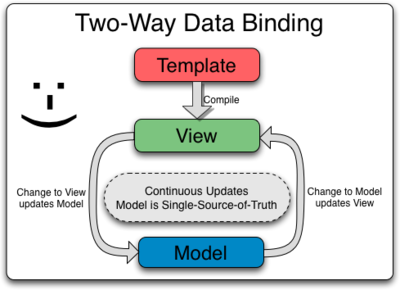
\includegraphics[width=8cm, keepaspectratio]{img/2waydatabinding}
    \caption{Funcionamiento del Two Way Data Binding}
    \label{fig:2waydatabinding}
\end{figure}

\subsubsection*{D3.js}
\label{subsec:d3}

La librer\'ia de JavaScript D3~\cite{d3}, llamada as\'i por las siglas Data-Driven Documents,
permite producir a partir de datos, gr\'aficos din\'amicos e interactivos mediante SVG.

\begin{figure}[H]
  \centering
  
\includegraphics[width=3cm, keepaspectratio]{img/d3-logo}
\end{figure}

Para este proyecto, utilizaremos D3 con otra librer\'ia basada en d3.js llamada nvd3.js, que permite
crear de manera sencilla y uniforme, gr\'aficos de distintos tipos y para cualquier
tipo de datos, que adem\'as se actualizan conforme estos datos vayan cambiando.

\subsection{HTML5 y CSS3}
\label{subsec:html5css3}

Para la realizaci\'on de este proyecto, juegan un papel importante tecnolog\'ias
como HTML5 o CSS3, que permiten la creaci\'on de una interfaz de usuario llamativa
y f\'acil para el correcto funcionamiento de la aplicaci\'on web.

\subsubsection*{HTML5}
\label{subsec:html5}

HTML5~\cite{html5} es un lenguaje de marcado que nos permite realizar plantillas en las que
representar nuestra interfaz de usuario.

\begin{figure}[H]
  \centering
  
\includegraphics[width=3cm, keepaspectratio]{img/html5-logo}
\end{figure}

Adem\'as el DOM de la p\'agina, que es una representaci\'on en \'arbol de los distintos
elementos de la plantilla HTML, nos permite modificar mediante distintas herramientas
como puede ser Angular, el aspecto y organizaci\'on de nuestra interfaz.

\subsubsection*{CSS3}
\label{subsec:css3}

Como complemento a HTML, tenemos CSS, que es un lenguaje creado para definir la presentaci\'on
y el estilo de documentos HTML o XML.

\begin{figure}[H]
  \centering
  
\includegraphics[width=3cm, keepaspectratio]{img/css3-logo}
\end{figure}

Mediante este lenguaje definiremos el estilo de nuestra interfaz de usuario, dot\'andola
de las caracter\'isticas deseadas para hacerla m\'as atractiva al usuario.

\subsection{Bootstrap}
\label{subsec:bootstrap}

Bootstrap~\cite{bootstrap} es un conjunto de herramientas de c\'odigo abierto, desarrollado y mantenido
por Twitter, que permite hacer nuestra p\'agina HTML/CSS responsiva. Es decir,
Bootstrap permite que una página web se adapte al tama\~no del navegador o el dispositivo en que
está siendo mostrada.

\begin{figure}[H]
  \centering
  
\includegraphics[width=4cm, keepaspectratio]{img/bootstrap-logo}
\end{figure}

Esta funcionalidad la otorga el sistema de celdas de Bootstrap que permite una
mejor maquetaci\'on de nuestra p\'agina web.

En este proyecto se utiliza Bootstrap por cuestiones est\'eticas, pero adem\'as por
seguir con la filosof\'ia de organizaci\'on y estructurac\'on del c\'odigo que se
asume al utilizar AngularJS.

\section{Control de versiones}
\label{sec:git}

Para la un mejor seguimiento y control de los avances de este proyecto, se ha
utilizado Git como herramienta de control de versiones.

\begin{figure}[H]
  \centering
  
\includegraphics[width=4cm, keepaspectratio]{img/git-logo}
\end{figure}

Este software fue dise\~nado por Linus Torvalds en 2005, para permitirle a el
y a su equipo un desarrollo m\'as \'agil y productivo.

Por este motivo y por la funci\'on de backup que estas versiones permiten,
se ha utilizado este software para registrar cada hito conseguido en el proyecto.

\section{Interacci\'on entre tecnolog\'ias}
\label{sec:interaction}

Por \'ultimo y para sintetizar, en esta secci\'on explicaremos las interacciones
entre las tecnolog\'ias descritas en las secciones anteriores.

Tal y como se muestra en la figura~\ref{fig:interaction}, al acceder un usuario
a la p\'agina web y realizar el an\'alisis o la b\'usqueda de ciertos datos, se enviar\'a
una petici\'on desde el cliente Angular hasta el servidor Django, que tras obtener
los datos de la base de datos, los devolver\'a en la respuesta al cliente, y este
actualizar\'a mediante el two way data binding los datos contenidos en los gr\'aficos
de la librer\'ia D3.

\begin{figure}[H]
    \centering
    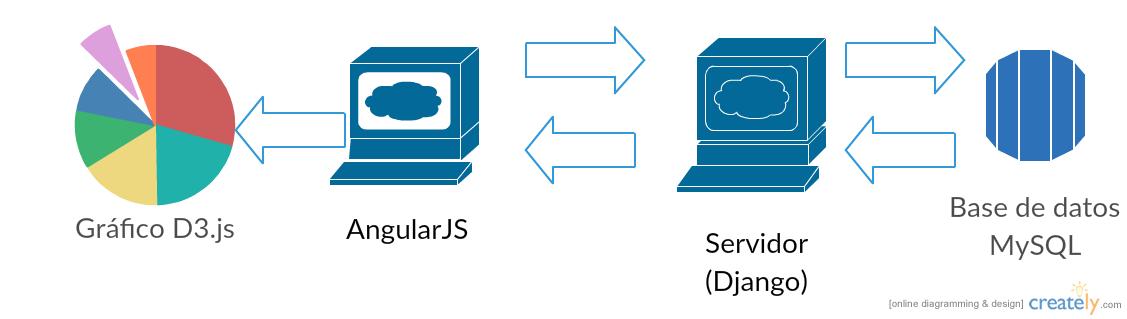
\includegraphics[width=12cm, keepaspectratio]{img/technologies-interaction}
    \caption{Interacci\'on entre las distintas tecnolog\'ias}
    \label{fig:interaction}
\end{figure}


%%%%%%%%%%%%%%%%%%%%%%%%%%%%%%%%%%%%%%%%%%%%%%%%%%%%%%%%%%%%%%%%%%%%%%%%%%%%%%%%
%%%%%%%%%%%%%%%%%%%%%%%%%%%%%%%%%%%%%%%%%%%%%%%%%%%%%%%%%%%%%%%%%%%%%%%%%%%%%%%%
% DISEÑO E IMPLEMENTACIÓN %
%%%%%%%%%%%%%%%%%%%%%%%%%%%%%%%%%%%%%%%%%%%%%%%%%%%%%%%%%%%%%%%%%%%%%%%%%%%%%%%%

\cleardoublepage
\chapter{Dise\~no e implementaci\'on}

En esta secci\'on se desarrollar\'a el proceso seguido para realizar el dise\~no
preliminar del proyecto y su implementaci\'on.

Primero se dar\'a una visi\'on general de la arquitectura de la aplicaci\'on para
posteriormente centrarse en las dos partes principales de la aplicaci\'on, el front-end
y el back-end, y debido a las diferentes tecnolog\'ias utilizadas en ambos, se
explicar\'a por \'ultimo el proceso de adaptaci\'on entre una y otra parte, para
el correcto funcionamiento de la aplicaci\'on.

\section{Arquitectura general}
\label{sec:arquitectura}

Este proyecto consiste en una aplicaci\'on web Django en la que se mostrar\'an los resultados
de un an\'alisis producido en el back-end de la aplicaci\'on.

El back-end o lado del servidor ha sido desarrollado en Python mediante el framework
web Django. En esta parte del c\'odigo se ha desarrollado una API REST que devolver\'a
en funci\'on de los recursos a los cuales se acceda, los resultados analizados en el
momento de la petici\'on o almacenados en la base de datos, del proyecto FOSS requerido
por el usuario. Adem\'as permitir\'a la obtenci\'on de los datos globales de la aplicaci\'on,
as\'i como los correspondientes a un usuario y aquellos relacionados con una determinada
inada
inforamci\'on legal.

De los resultados devueltos por el servidor se servir\'a el c\'odigo del navegador
o front-end. Este c\'odigo realizar\'a funciones de visualizaci\'on de los datos
obtenidos. Mediante el framework web AngularJS se realizar\'a una SPA que mostrar\'a
dos secciones en las que visualizar los datos, una en la que analizar un proyecto
y otra en la que visualizar las estad\'isticas totales almacenadas en la base de datos,
adem\'as de poder filtrarlas.

Para una mejor comprensi\'on de la aplicaci\'on, se desarrollar\'a en mayor profundidad
el funcionamiento de la misma en los siguientes apartados.

%figura~\ref{fig:arquitectura}.

%\begin{figure}
%  \centering
%  \includegraphics[width=9cm, keepaspectratio]{img/arquitectura}
%  \caption{Estructura del parser b\'asico}
%  \label{fig:arquitectura}
%\end{figure}


\section{Back-end}
\label{sec:back-end}

En este apartado se explicar\'an las caracter\'isticas de la API REST desarrollada
en el servidor Django.

Para implementar esta aplicaci\'on y esta API REST, se puso en funcionamiento
primero un proyecto Django sobre el cual se desarrollar\'a el back-end de la aplicaci\'on.

Desde este servidor Django se sirven los archivos correspondientes a la p\'agina
principal y en este caso \'unica de la aplicaci\'on, adem\'as del c\'odigo correspondiente
al funcionamiento de la p\'agina. Tambi\'en en este servidor se puede acceder a
cuatro recursos diferentes correspondientes a la API REST ya mencionada.

Estos recursos son los siguientes:

\begin{itemize}
  \item \textbf{/analyze}: Accediendo a este recurso y enviando en el cuerpo de
  la petici\'on HTTP, la url de un proyecto, se obtienen los datos correspondientes
  al an\'alisis del proyecto al que corresponde la url. Entre estos datos se
  encuentran los ficheros que contiene y los contribuidores, las licencias y los
  copyrights presentes en ellos.

  \item \textbf{/all}: Mediante el acceso a este recurso se devolver\'an en la
  respuesta todos los datos contenidos en la base de datos que hagan referencia
  al total de lineas que ha desarrollado cada contribuidor, los lenguajes utilizados
  y los copyrights y licencias utilizados en los distintos ficheros almacenados.

  \item \textbf{/user}: Al realizar una petici\'on HTTP sobre este recurso con
  el nombre de un usuario en su cuerpo, se devolver\'an los lenguajes utilizados
  por este usuario, los proyectos en los que ha participado y las licencias y
  copyrights que ha utilizado en sus ficheros.

  \item \textbf{/legal}: Al acceder a este recurso, se podr\'an enviar una licencia
  o un copyright por los cual se quieran filtrar los ficheros almacenados en la
  base de datos, devolviendo en la respuesta todos los ficheros que contengan
  esta informaci\'on legal.

\end{itemize}

\subsection{An\'alisis de proyectos}
\label{subsec:analysis}

A continuaci\'on se describir\'a el proceso de an\'alisis de los distintos proyectos
as\'i como la implementaci\'on de dicho an\'alisis.

\subsubsection*{Proceso}
\label{subsubsec:proceso}

El an\'alisis se realizar\'a al acceder al recurso /analyze
siempre y cuando no haya sido almacenado previamente en la base de datos, y la
fecha en la que fue almacenado sea m\'as reciente que la fecha de \'ultima
modificaci\'on del proyecto.

Si se cumplen estas dos condiciones, en la vista correspondiente al recurso /analyze
se utilizar\'a la librer\'ia GitPython para clonar el repositorio del proyecto
a analizar, para posteriormente utilizar la herramienta Scancode Toolkit sobre la
carpeta en la que este proyecto fue clonado.

Mediante esta herramienta finalmente se obtendr\'a la informaci\'on legal de cada
fichero, y mediante la librer\'ia GitPython y la API de Github se obtendr\'a otra informaci\'on como
pueden ser los contribuidores y las contribuciones de cada uno de ellos.

\subsubsection*{Implementaci\'on}
\label{subsubsec:implementacion}

Para implementar este proceso se har\'a uso de una funci\'on que con la herramienta
Scancode Toolkit, recorrer\'a todos los archivos contenidos en la carpeta para
obtener de cada uno de ellos sus licencias y copyrights. Esta herramienta utiliza
una lista de licencias y reglas que le sirven como patr\'on para comparar el
contenido de cada fichero en busca de las licencias a las que correspondan dichas reglas.

Adem\'as de Scancode, se utilizar\'a como se especific\'o anteriormente, la API de
Github, que devuelve un objeto JSON con la informaci\'on requerida, en este caso
los contribuidores e informaci\'on general del proyecto.

Por otro lado, tambi\'en se utilizan GitPython para obtener las lineas equivalentes al comando git blame de Git,
que ser\'an posteriormente parseadas para obtener el autor de cada una y la biblioteca
Pygments que a partir del contenido de cada fichero, determinar\'a el lenguaje en
que est\'a programado en base a su sintaxis.

\subsubsection*{Otras consideraciones}
\label{subsubsec:consideraciones}

Para el correcto funcionamiento de la aplicaci\'on fueron necesarias ciertas modificaciones
sobre la herramienta Scancode Toolkit:

\begin{itemize}
\item El funcionamiento por defecto de Scancode Toolkit carga la lista de reglas
y licencias en cada an\'alisis. En este caso, al tratarse de una aplicaci\'on web,
esta funcionalidad no es viable, por lo tanto se tuvo que modificar el
funcionamiento de la herramienta para que la carga de licencias se realice
nada m\'as arrancar la aplicaci\'on web, almacenando despu\'es la lista en el
servidor, y evitando as\'i que se tengan que realizar cargas posteriores.

\item Para facilitar el an\'alisis completo de los proyectos se decidi\'o leer
el contenido de los distintos ficheros al comenzar el proceso de an\'alisis,
evitando as\'i, las distintas lecturas que habr\'ia que realizar por defecto en el
funcionamiento de las herramientas utilizadas. De esta forma, para evitar estas
m\'ultiple lecturas, se modific\'o la herramienta Scancode Toolkit para poder
analizar el contenido de cada fichero directamente en lugar de leerlo dentro
del c\'odigo de esta herramienta.

\end{itemize}

\subsection{Procesado de estad\'isticas}
\label{subsec:statistics}

En esta secci\'on se describir\'an los procesos de obtenci\'on y env\'io de los datos
estad\'isticos de los proyectos, adem\'as de su filtrado.

\subsubsection*{Tablas de la base de datos}
\label{subsubsec:tablas_bd}

La obtenci\'on de los datos de la base de datos de MySQL se realizar\'a mediante
el uso de los modelos que nos da la funcionalidad de Django. De esta manera, al
acceder a los recursos /all, /user o /legal, se realizar\'an las interacciones
necesarias con la base de datos gracias a la sencilla interfaz que nos proporcionan
estos modelos.

Es necesario destacar que al tratarse de una base de datos relacional, se tendr\'a
que acceder a las distintas tablas a las cuales pertenecen los datos de estas
relaciones, antes de elaborar la respuesta.

La disposici\'on de las tablas presentes en la base de datos, adem\'as de las
distintas relaciones entre ellas se puede observar en la figura~\ref{fig:database}.

\begin{figure}
  \centering
  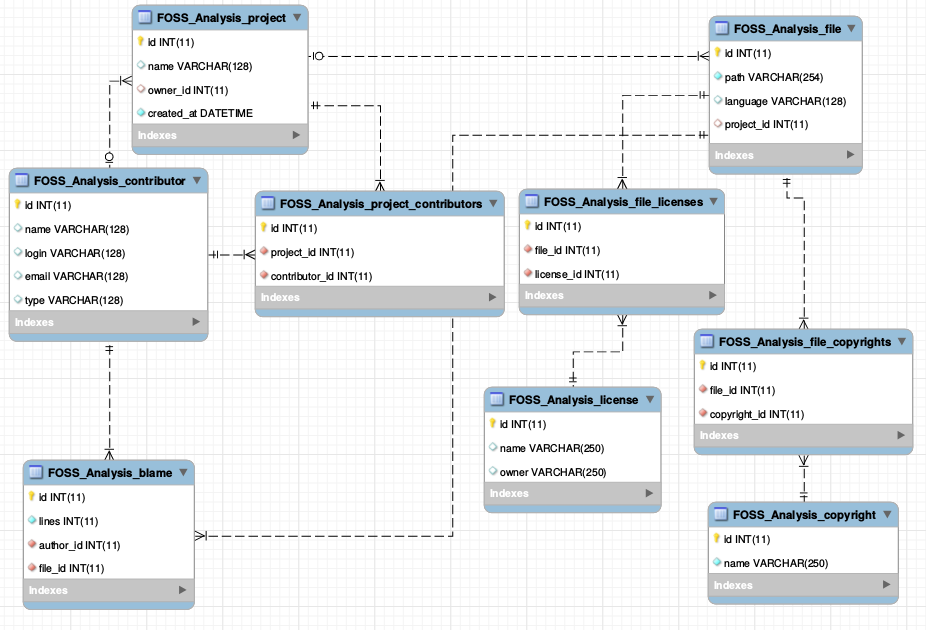
\includegraphics[width=14cm, keepaspectratio]{img/mysql_tables}
  \caption{Distribuci\'on de la base de datos}
  \label{fig:database}
\end{figure}

En esta figura observamos las siguientes tablas de la base de datos:

\begin{itemize}

\item \textbf{Project}: En esta tabla contiene el nombre y la fecha de almacenamiento
del proyecto, adem\'as del due\~no y los contribuidores del proyecto mediante unas relaciones
de Foreign Key y Many to Many respectivamente con la tabla de Contributor.

\item \textbf{Contributor}: Donde se almacena el nombre, login e email del contribuidor,
teniendo adem\'as el par login, email como clave \'unica de los contribuidores, de forma
que no podr\'an almacenarse dos contribuidores cuyos campos de login y email sean
ambos iguales.

\item \textbf{File}: Para almacenar los ficheros contenidos en cada proyecto
utilizaremos esta tabla, donde se almacenan el path absoluto donde ha sido analizado
el fichero y el lenguaje en que este est\'a programado. Adem\'as de esto, esta tabla
estar\'a relacionada con las tablas Project, Copyright y License para determinar
ar
a que proyecto pertenece el archivo y que copyrights y licencias est\'an contenidas
en el.

\item \textbf{Blame}: En la tabla Blame se almacenar\'an las contribuciones por cada
fichero que ha realizado cada usuario. Esto se realizar\'a almacenando las lineas de
c\'odigo que cada contribuidor ha realizado, guardando el id correspondiente con
el contribuidor en la tabla Contributor en el campo author, y as\'i mismo
con el fichero en el campo file.

\item \textbf{Copyright}: Donde se almacena el nombre del copyright y a quien pertenece.

\item \textbf{License}: Donde se guardan los nombres de las distintas licencias.

\end{itemize}

\subsubsection*{Queries}
\label{subsubsec:queries}

Una vez descrito el modo en que est\'an almacenados los datos en las distintas
tablas de MySQL, procedemos a describir las interacciones que se han de realizar
con la base de datos para poder obtener y enviar los distintos datos.

\paragraph*{Estad\'isticas de proyecto}
\label{paragraph:project_stats}

Para la obtenci\'on de los datos globales de cada proyecto accederemos al recurso
/analyze en cuya vista se realizar\'a una query sobre la tabla de proyectos en la
que se traer\'an adem\'as los datos relacionados con la tabla de contribuidores.

Tras realizar esta query se procesar\'an los datos para que sean serializables
y para que tengan un formato JSON aceptable para el front-end programado en JavaScript.

\paragraph*{Estad\'isticas totales}
\label{paragraph:total_stats}

En el caso de la obtenci\'on del total de los datos almacenados en la base de datos,
se realizar\'an tres queries distintas sobre la tabla File, de las que se obtendr\'an
los datos relacionados de las licencias y copyrights de todos los ficheros, adem\'as
de los datos del lenguaje de cada uno de ellos. Por \'ultimo, se har\'a una petici\'on sobre
la tabla Blame que devolver\'a el n\'umero de lineas totales realizadas por cada autor en
los distintos ficheros.

Sobre estos datos se realizar\'a una suma mediante el m\'etodo count de SQL para cada valor diferente,
gracias al m\'etodo de la interfaz que aporta Django con el mismo nombre. Obteniendo
as\'i el numero total de lineas realizadas por cada autor y el n\'umero total de
copyrights, licencias y lenguajes diferentes.

Por \'ultimo se procesar\'an los datos para adaptarlos al formato JSON, y adem\'as
al formato de los datos que tendr\'an que ser introducidos en los gr\'aficos de D3.

\paragraph*{Estad\'isticas de usuario}
\label{paragraph:user_stats}

Para obtener los datos concretos de un usuario, sobre la tabla Blame se realizar\'an
tres peticiones para obtener el n\'umero total de ficheros programados en cada lenguaje,
y que contienen cada tipo de copyright y licencia, filtr\'andolos por el usuario determinado.
Adem\'as se har\'an dos queries en las que se obtendr\'an todos los nombres de proyectos
en los que el usuario participa como due\~no o como colaborador del mismo.

Este filtrado se realizar\'a mediante el m\'etodo where del lenguaje SQL o en este
caso, del m\'etodo filter de la API de Django models.

Al igual que en el caso anterior, se realizar\'a un procesado final antes de enviar
la respuesta con los datos obtenidos, filtrados y sumados.

\paragraph*{Estad\'isticas legales}
\label{paragraph:legal_stats}

Por \'ultimo se obtendr\'an todos los ficheros filtrados por licencias o por
copyrights.

En este caso se realizar\'a un filtrado como en el caso anterior, pero con la
diferencia de que en este caso se filtrar\'a de manera no estricta, es decir,
valdr\'a con introducir una palabra contenida en los copyrights o licencias del fichero,
para que este sea devuelto en la respuesta.


\section{Front-end}
\label{sec:front-end}

A continuaci\'on se pasar\'a a explicar el funcionamiento y dise\~no de la parte
del cliente de la aplicaci\'on.

Como ya se ha comentado antes, esta secci\'on del proyecto est\'a implementada
con el framework AngularJS, el cual aporta una estructura al c\'odigo que se
pasar\'a a explicar a continuaci\'on.

\subsection{Estructura AngularJS}
\label{subsec:angular_structure}

El framework Angular nos permite s permite dividir nuestro c\'odigo por m\'odulos, los
cuales permitir\'an diferenciar de manera adecuada las distintas funcionalidades
que pueda tener nuestra web. Los m\'odulos que forman esta aplicaci\'on son los
siguientes:

\begin{itemize}

\item \textbf{Main}: Permite la selecci\'on de las distintas secciones de la p\'agina
sin necesidad de recargar o acceder a una nueva url, convirtiendo as\'i la p\'agina
en una Single Page Application.

\item \textbf{An\'alysis}: Accediendo a la API implementada en el servidor Django,
obtiene los datos analizados del proyecto, y los almacena de modo que puedan ser usados
por la plantilla HTML correspondiente a este m\'odulo y sus gr\'aficos.

\item \textbf{Statistics}: En este m\'odulo al igual que en el de Analysis se
obtendr\'an los datos de la API del servidor, y se mostrar\'an en tres plantillas
diferentes ya sean datos totales, de usuario o legales.

\item \textbf{Navbar}: Es el m\'odulo que permite controlar el funcionamiento de
la barra de navegaci\'on, permitiendo mostrar las secciones que contiene la p\'agina.

\item \textbf{Chart}: El m\'odulo de Chart se crear\'an los gr\'aficos que nos
servir\'an para representar los datos de los m\'odulos de Analysis y Statistics.
Por tanto estos dos m\'odulos tendr\'an una dependencia con el de Chart.

\end{itemize}

Todos estos m\'odulos se inyectan en las dependencias del m\'odulo principal de
la aplicaci\'on, que ser\'a el m\'odulo app.

\subsection{Funcionamiento}
\label{subsec:angular_funcionamiento}

En los distintos m\'odulos se establecer\'an una serie de directivas Angular
que permitir\'an el intercambio de los distintos parciales o plantillas HTML,
gracias a la colocaci\'on del m\'etodo ng-view en un elemento del DOM.
Mediante este m\'etodo, en este elemento se colocar\'an los contenidos de las
plantillas referenciadas dentro de cada directiva.

Una vez mostrada la plantilla correspondiente a cada directiva, se permitir\'a
mediante distintos formularios, la realizaci\'on de peticiones de datos a la base
de datos tal y como se ha explicado anteriormente.

Tras obtener la respuesta a las peticiones, se almacenar\'a en campos del elemento
\textdollar scope de Angular, permitiendo mediante el Two Way Data Binding ya mencionado,
la actualizaci\'on y representaci\'on de los datos en cada plantilla.

Cabe mencionar, que en el caso de los gr\'aficos de la biblioteca D3 es necesario
actualizar el gr\'afico con los nuevos datos. Este proceso no es autom\'atico,
por tanto se ha hecho uso del m\'etodo \textdollar watch para a\~nadir un manejador al evento de
actualizaci\'on de los datos, as\'i cuanto este evento se produzca, se llamar\'a
a una funci\'on que generar\'a el gr\'afico de nuevo y actualizado con los nuevos
datos.

\section{Adaptaci\'on de la informaci\'on}
\label{sec:adaptation}

Debido a las distintas tecnolog\'ias utilizadas en el back-end y en el front-end,
donde se utilizan Python y JavaScript respectivamente, se producen ciertas incompatibilidades
entre los formatos de uno y otro extremo.

Estos conflictos no suponen un problema a la hora de realizar ambas partes por
separado, pero es necesario atajarlos ya que entre uno y otro punto se produce
un intercambio de informaci\'on.

En este caso, al ser JavaScript, en el front-end, el consumidor de la informaci\'on,
ser\'a necesario que antes de su env\'io, la informaci\'on sea procesada para darle
un formato JSON. Este formato implica tener una colecci\'on de elementos con una
clave y un valor asociado a ella.

Este formato permitir\'a una adecuada serializaci\'on desde el servidor al cliente
para el correcto env\'io de la respuesta, y que en el front-end no se requiera ning\'un
procesado especial de la respuesta, m\'as que el de un elemento JSON propio de JavaScript,
y su posterior adaptaci\'on para su representaci\'on.

La adaptaci\'on de la informaci\'on supone un elemento clave tambi\'en para considerar
la API desarrollada como una API REST, puesto que esto conlleva una homogeneidad entre los
recursos y el formato JSON permite dar esta homogeneidad a las respuestas de estos recursos.

%%%%%%%%%%%%%%%%%%%%%%%%%%%%%%%%%%%%%%%%%%%%%%%%%%%%%%%%%%%%%%%%%%%%%%%%%%%%%%%%
%%%%%%%%%%%%%%%%%%%%%%%%%%%%%%%%%%%%%%%%%%%%%%%%%%%%%%%%%%%%%%%%%%%%%%%%%%%%%%%%
% RESULTADOS %
%%%%%%%%%%%%%%%%%%%%%%%%%%%%%%%%%%%%%%%%%%%%%%%%%%%%%%%%%%%%%%%%%%%%%%%%%%%%%%%%

\cleardoublepage
\chapter{Resultados}

Una vez enumerado el proceso de an\'alisis, se proceder\'a a mostrar los resultados
obtenidos del an\'alisis de proyectos pertenecientes a repositorios Github de
mayor o menor relevancia.

\section{Interfaz de usuario}
\label{sec:user_interface}

Primero se mostrar\'a la interfaz de usuario de la aplicaci\'on en la que se representar\'an
los datos que se enumerar\'an en las secciones siguientes.

En los dos primeros gr\'aficos se mostrar\'an los lenguajes utilizados y los colaboradores
m\'as activos tal y como se muestra en la figura~\ref{fig:first_row}.

\begin{figure}
  \centering
  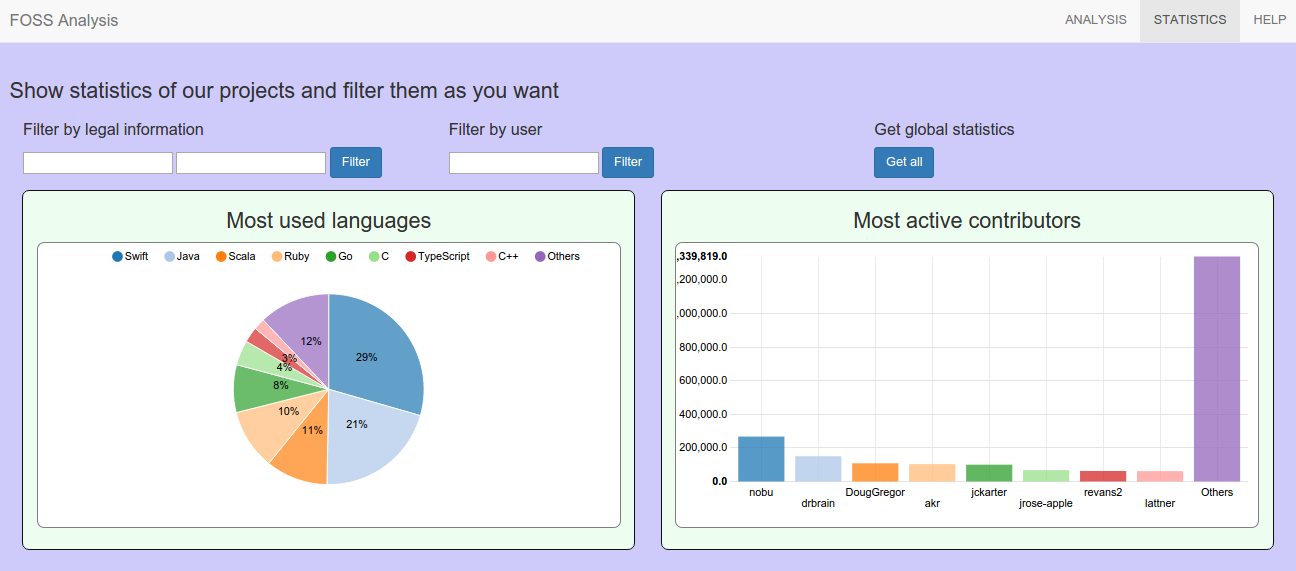
\includegraphics[width=12cm, keepaspectratio]{img/first_row}
  \caption{Gr\'aficos de lenguajes y contribuidores}
  \label{fig:first_row}
\end{figure}

En la segunda secci\'on, mostrada en la figura~\ref{fig:second_row} de gr\'aficos se mostrar\'an
las licencias y copyrights presentes en el proyecto.

\begin{figure}
  \centering
  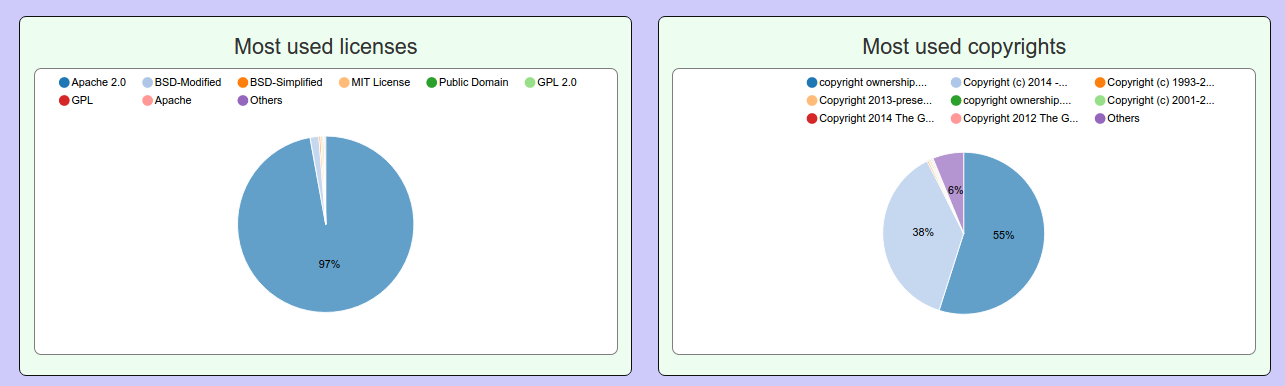
\includegraphics[width=12cm, keepaspectratio]{img/second_row}
  \caption{Gr\'aficos de licencias y copyrights}
  \label{fig:second_row}
\end{figure}

Y por \'ultimo, en la tercera secci\'on se mostrar\'a una lista con el desglose de todos
los ficheros con su datos individuales. Esta secci\'on se muestra en la figura~\ref{fig:third_row}

\begin{figure}
  \centering
  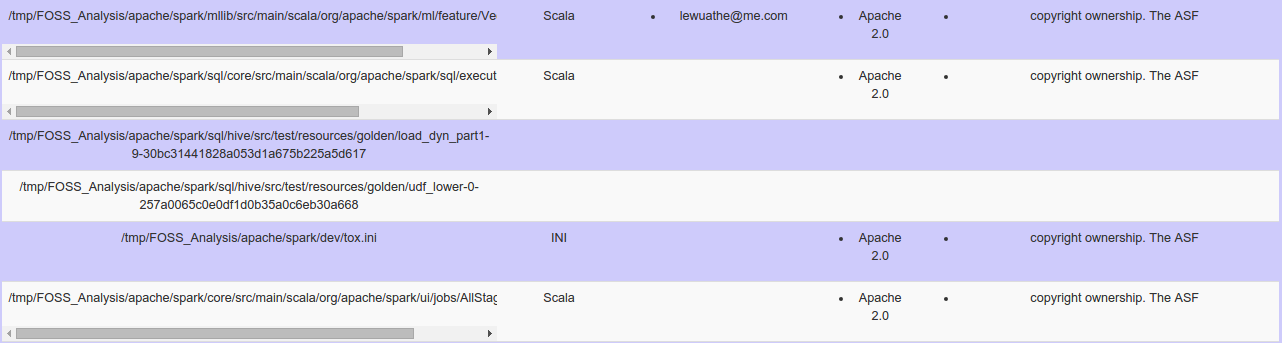
\includegraphics[width=12cm, keepaspectratio]{img/row_third}
  \caption{Lista de ficheros}
  \label{fig:third_row}
\end{figure}

Para mostrar unos resultados reales en esta interfaz, se analizar\'an distintos proyectos populares entre
la comunidad de Free Open Source Software. Entre estos proyectos se han elegido los
repositorios de herramientas como Docker, Ruby, Swift, React, Apache/Storm, Apache/Spark,
Scala, Go, etc.

\section{Informaci\'on general}
\label{sec:general_info}

En los distintos proyectos analizados, se puede comprobar una serie de caracter\'isticas
comunes que var\'ian muy poco de uno a otro, no obstante, la informaci\'on obtenida de
estas peque\~nas diferencias nos sirve para analizar el entorno en que estos proyectos
han sido realizados. En este apartado se describir\'an las propiedades generales que
comparten todos estos proyectos.

Para analizar estos proyectos se ha recurrido a la plataforma Github en la que se puede
acceder a sus repositorios. El hecho de que est\'en presentes de manera p\'ublica
en una plataforma en la que el c\'odigo es totalmente accesible, muestra las caracter\'isticas
Free Open Source de dichos proyectos.

Estas propiedades Free Open Source se aprecian tambi\'en en la variedad de licencias utilizadas.
Aunque no todos los proyectos utilicen las mismas licencias, la mayor\'ia de ellas son permisivas
y cumplen las cuatro libertades del software libre, de uso, de modificaci\'on, de distribuci\'on
y de mejora.

Por otra parte, la mayor\'ia de estos proyectos pertenecen a grandes empresas del sector tecnol\'ogico, que
a pesar de ser lucrativas, han visto en el ecosistema Free Open Source el futuro del desarrollo software.
Debido a la gran comunidad de desarrolladores presentes en este entorno, las empresas se benefician
de la colaboraci\'on de programadores de todo el mundo para mejorar su software, de esta forma,
observamos un n\'umero de contribuidores muy elevado, y por consiguiente, un crecimiento de
las dimensiones del proyecto proporcional a este n\'umero.

Esta es otra caracter\'istica fundamental de todos los proyectos FOSS si quieren ser fruct\'iferos, la comunidad.
Por un lado las empresas se benefician de la contribuci\'on de distintos colaboradores a los cuales incluso
podr\'ian reclutar, y por otro, los contribuidores desarrollan tanto su carrera como sus habilidades program\'aticas.

Por \'ultimo, adem\'as, de todas estas peculiaridades de los proyectos FOSS, se ha de destacar la reutilizaci\'on y
mejora de herramientas y proyectos a la hora de desarrollar un nuevo software. Todos los proyectos analizados,
basan su funcionamiento en otro software, ya sean lenguajes de programaci\'on, herramientas web, herramientas para
la distribuci\'on de aplicaciones, etc. Lo cual hace de la colaboraci\'on de la comunidad, un factor imprescindible
para que un proyecto de software libre tenga \'exito.

A continuaci\'on se enumerar\'an las cualidades espec\'ificas de diferentes proyectos analizados.

\section{Informaci\'on espec\'ifica de los proyectos}
\label{sec:specific_info}

En esta secci\'on se enumerar\'an los resultados obtenidos para tres tipos diferentes de proyectos,
para herramientas de desarrollo software como son Angular y Docker, para lenguajes de programaci\'on como
Ruby y Swift y por \'ultimo, para el repositorio del Kernel de Linux.

\subsection{Herramientas para el desarrollo software}
\label{subsec:software_tools}

Docker y Angular son dos herramientas de software libre cuyas funciones son de plataforma para aplicaciones distribuidas
y framework web respectivamente.

Estas dos herramientas difieren en su funcionalidad, pero no tanto en sus caracter\'isticas Free Open Source.
Ambos proyectos usan en la pr\'actica la licencia BSD-Modified mayoritariamente, como se muestra en las
figuras~\ref{fig:angular_license} y~\ref{fig:docker_license}. Ya que aunque AngularJS presenta un 60% de sus archivos licenciados
bajo la licencia MIT, al ser esta una licencia muy permisiva, y permitir ser incorporada bajo otras licencias,
en Angular se hace uso de la licencia BSD la cual es m\'as restrictiva que la MIT License.

\begin{figure}
  \centering
  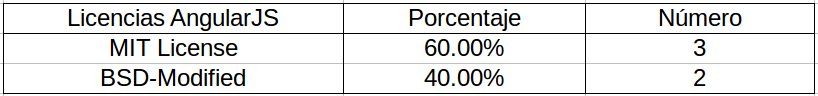
\includegraphics[width=14cm, keepaspectratio]{img/licenses_angular}
  \caption{Licencias presentes en AngularJS}
  \label{fig:angular_license}
\end{figure}

\begin{figure}
  \centering
  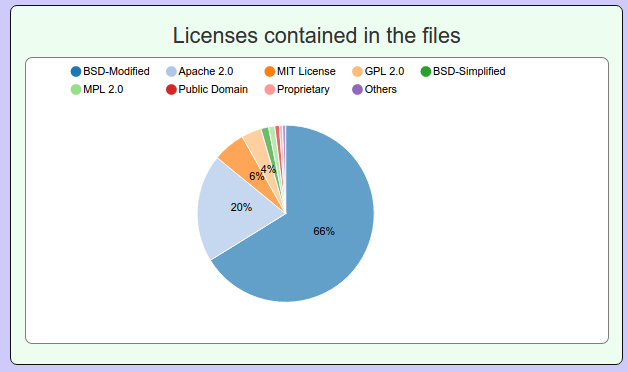
\includegraphics[width=14cm, keepaspectratio]{img/licenses_docker}
  \caption{Licencias presentes en Docker}
  \label{fig:docker_license}
\end{figure}

Los permisos que se otorgan a ambos proyectos mediante la licencia BSD-Modified son los siguientes:

\begin{itemize}
	\item \textbf{Uso comercial}: Permiso para utilizar el c\'odigo con prop\'ositos comerciales y lucrativos.

	\item \textbf{Modificaci\'on}: Permiso para modificar y crear proyectos derivados del c\'odigo que al que da licencia.

	\item \textbf{Distribuci\'on}: Permiso para distribuir el c\'odigo original o cualquier derivado del mismo.

	\item \textbf{Compatibilidad de licencias}: La licencia BSD es compatible con cualquier otra licencia de software libre.
\end{itemize}

Adem\'as, la licencia MIT otorga permisos de utilizar AngularJS para uso privado.

Por otro lado, la licencia BSD-Modified restringe el uso del c\'odigo de los siguientes modos:

\begin{itemize}
	\item \textbf{Uso de Trademarks}: No se permite usar el nombre de empresas o marcas registradas en el c\'odigo
	para ratificar o beneficiar la popularidad de un trabajo derivado del original, perteneciente a esa empresa o marca registrada.

	\item \textbf{Responsabilizaci\'on}: No se responsabilizar\'a al autor del software por ning\'un perjuicio ocasionado.

	\item \textbf{Inclusi\'on de copyright}: Se deber\'a conservar siempre en el c\'odigo original y en su uso
	en cualquier c\'odigo derivado, el copyright original del mismo.

	\item \textbf{Inclusi\'on de licencia}: Se deber\'a conservar siempre el texto completo de la licencia BSD.
\end{itemize}

Estas restricciones salvo la del uso de Trademarks se aplican tambi\'en a trav\'es de la licencia MIT en el caso de Angular.
Pero al usarse las licencias MIT y BSD conjuntamente se aplican las restricciones de ambas si aparecen las dos en el c\'odigo
como es el caso del proyecto Angular.

Adem\'as de las licencias, cabe destacar el uso de determinados lenguajes en estas herramientas. Por un lado, Docker utiliza
Go como lenguaje principal tal y como se muestra en la figura~\ref{fig:docker_lang}, este lenguaje es tambi\'en Free Open Source,
contando con una licencia BSD modificada, que le otorga a Google, su distribuidor, un derecho de patente sobre el lenguaje,
pero sin que esto suponga un recorte en los derechos de utilizaci\'on de Go por parte de Docker.

\begin{figure}
  \centering
  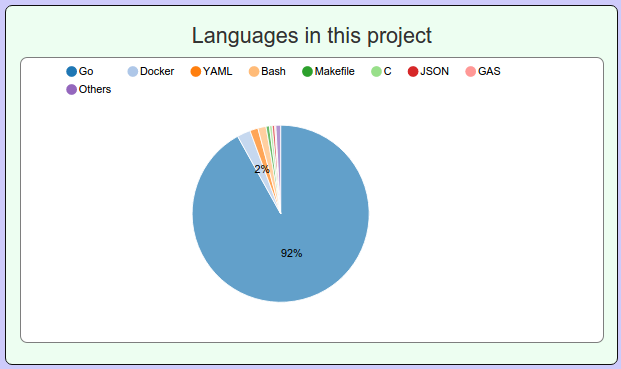
\includegraphics[width=14cm, keepaspectratio]{img/languages_docker}
  \caption{Lenguajes utilizados por Docker}
  \label{fig:docker_lang}
\end{figure}

Por otro lado, en Angular los principales lenguajes de programaci\'on son TypeScript y Dart, que utilizan licencias Apache
y BSD respectivamente tal y como se ve en la figura~\ref{fig:angular_lang}. En este caso, las dos, al igual que en el caso de Docker,
son licencias libres. Y Apache al igual que en el caso anterior, otorga derecho de patente a Microsoft sobre TypeScript
sin que esto suponga una p\'erdida de derechos por parte de Google sobre Angular.

\begin{figure}
  \centering
  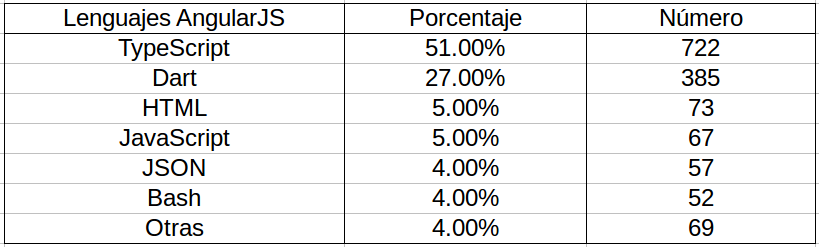
\includegraphics[width=14cm, keepaspectratio]{img/languages_angular}
  \caption{Lenguajes utilizados por AngularJS}
  \label{fig:angular_lang}
\end{figure}

%Bibliografia licencias y compatibilidad entre licencias

\subsection{Repositorios de lenguajes de programaci\'on}
\label{subsec:languages_repos}

Adem\'as del an\'alisis de herramientas concretas y de m\'as alto nivel, se decidi\'o analizar tambi\'en proyectos
correspondientes a lenguajes de programaci\'on para, adem\'as de ver sus car\'acteristicas legales en cuanto
si son libres y abiertos, conocer los lenguajes y herramientas en los que se basan a su vez estos lenguajes.

Los lenguajes seleccionados, por ser relativamente modernos y con un nivel de abstracci\'on superior a los que daban
lenguajes como C o C++, son Ruby y Swift.

Ruby por su parte es un lenguaje dise\~nado y desarrollado por Yukihiro Matsumoto en 1995 y que tal y como se puede ver
en la figura~\ref{fig:ruby_lang}, consta de una serie de ficheros escritos en Ruby que corresponden con librer\'ias y funcionalidad
espec\'ifica del lenguaje, pero una vez observamos el c\'odigo del propio lenguaje, podemos comprobar que este est\'a programado
en C. Esta situaci\'on se da en la mayor\'ia de lenguajes modernos, que se basan en C, C++ y sus derivados, debido
a la libertad de uso que estos proporcionan, permitiendo al desarrollador controlar todos los aspectos de su software.
Utilizando este lenguaje como interprete, se otorga al nuevo lenguaje, en este caso Ruby, un mayor nivel de abstracci\'on
que a pesar de restringir la libertad en su uso, proporciona una mayor simplicidad al mismo.

\begin{figure}
	\centering
	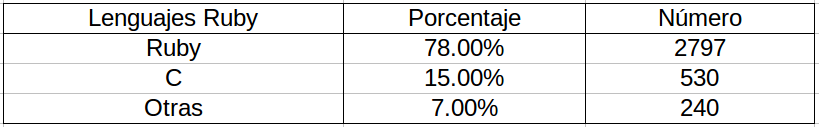
\includegraphics[width=14cm, keepaspectratio]{img/languages_ruby}
	\caption{Lenguajes utilizados en el proyecto Ruby}
	\label{fig:ruby_lang}
\end{figure}

Por otro lado tenemos el caso de Swift. Swift es un lenguaje de programaci\'on desarrollado por Apple que fue software
propietario hasta su versi\'on 2.2 y que al igual que Ruby tiene una librer\'ia est\'andar programada en Swift y cuya
base est\'a escrita en C++.

Tal y como se puede observar en la figura~\ref{fig:swift_license}, el 100% de sus licencias son Apache 2.0, que
otorga derechos de patente al desarrollador. En casos anteriores ya ha aparecido esta licencia. En aquellos casos,
la licencia no afectaba a la herramienta que utilizaba ese lenguaje de programaci\'on porque
se restring\'ia \'unicamente a su uso, y en ning\'un momento modificaba el c\'odigo de dicho lenguaje.
En caso de que se quisiera modificar Swift, cualquier modificaci\'on realizada sobre el c\'odigo supondr\'ia que
el colaborador tiene que dar una licencia a todos los usuarios de cualquier patente que pueda poseer sobre esa
colaboraci\'on.

\begin{figure}
	\centering
	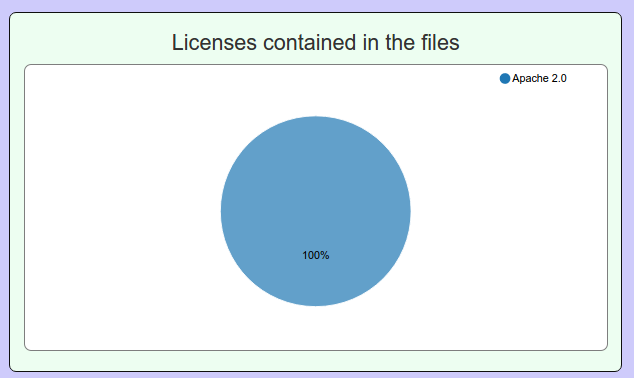
\includegraphics[width=14cm, keepaspectratio]{img/licenses_swift}
	\caption{Licencias presentes en el proyecto Swift}
	\label{fig:swift_license}
\end{figure}

Esta restricci\'on mitiga el problema de las patentes en el desarrollo de software libre, evitando que si alguien
intenta apropiarse de una patente mediante un tr\'amite legal, sean revocados sus derechos de patente sobre todo
el software o sobre las secciones de software en las cuales colabor\'o.

Este tipo de licencias est\'an proliferando m\'as \'ultimamente, para ayudar a grandes empresas como Apple o Google,
a sentirse m\'as c\'omodas al hacer que su software pertenezca a la comunidad Free Open Source.

\subsection{Herramientas de Big Data}
\label{subsec: big_data}

Por \'ultimo, se mostrar\'an a continuaci\'on los resultados obtenidos del an\'alisis de dos proyectos de software de
mayor actualidad, los proyectos de Apache Spark y Apache Flink. Estos proyectos se engloban dentro del \'ambito del
desarrollo software llamado Big Data y se utilizan para el procesado de grandes cantidades de streams de datos, para
aprendizaje m\'aquina, etc.

Al ser Big Data un tema muy actual, estas herramientas contienen, adem\'as de por pertenecer a la Apache Software
Foundation, licencias Apache 2.0 en la gran mayor\'ia de su c\'odigo. Esto aplica a estos proyectos el derecho
de patente para todos sus colaboradores.

Por otro lado, si analizamos los lenguajes utilizados en estos dos proyectos, comprobamos
que ambos contienen, en su mayor\'ia, c\'odigo escrito en Java y Scala, estos dos lenguajes
son muy comunes en el an\'alisis de grandes cantidades de datos. Por su simplicidad
y escalabilidad, Scala se ha convertido en uno de los lenguajes de programaci\'on
principales para el desarrollo de herramientas de Big Data.

\section{Lenguajes utilizados}
\label{sec:languages}

En la secci\'on anterior se han explicado los datos obtenidos para tres conjuntos
diferentes de proyectos de software libre. A partir de ese an\'alisis podemos estudiar
el uso de diferentes tipos de lenguajes en funci\'on de las cualidades y objetivos del
proyecto analizado.

En el caso de proyectos que implementan nuevos lenguajes de programaci\'on se observa
el uso generalizado de C, C++ y sus derivados, al ser estos lenguajes de programaci\'on
de bajo nivel, que permiten implementar interfaces entre los procesos y el control de
la memoria propios de lenguajes como C, para que el nuevo lenguaje alcance un mayor grado de abstracci\'on.

Si observamos, por otra parte, proyectos relacionados con herramientas de m\'as alto
nivel de abstracci\'on, como frameworks, plataformas para la distribuci\'on de aplicaciones, herramientas
de Big Data o machine learning, requerir\'an del uso de lenguajes de programaci\'on de alto
nivel como pueden ser Ruby, Python, Go, Scala, JavaScript e incluso Java.

Adem\'as, en funci\'on de las necesidades de la herramienta como ya se ha mostrado,
predominar\'a el uso de un lenguaje u otro. De esta forma, para frameworks web en el
front-end se suele utilizar JavaScript, para an\'alisis de Big Data se suele
utilizar Scala por su escalabilidad y para proyectos de machine learning se suele
utilizar Python entre otros por el gran n\'umero de librer\'ias que presenta el
lenguaje para este prop\'osito.

A continuaci\'on se enumerar\'an las consecuencias que podemos extraer de los datos
anteriormente recogidos.

\section{Consecuencias extra\'idas}
\label{sec:consecuencias}

Tras la obtenci\'on de los datos anteriores, se pudo comprobar la importancia del software libre en el desarrollo de los nuevos
proyectos de software, ya sea para empresas con \'animo de lucro o desarrolladores particulares. El mundo del desarrollo software
se basa en la comunidad, en la reutilizaci\'on de herramientas y en el intercambio de conocimientos para alcanzar los
objetivos marcados en cada proyecto.

Al analizar los proyectos mencionados en la secci\'on \ref{sec:specific_info} se ha obtenido una mejor visi\'on de las libertades que proporciona
el software libre y los matices que existen dentro del mismo, porque aunque todo el software analizado sea
libre, las diferentes licencias analizadas, otorgan ciertas cualidades diferentes a cada proyecto.

La principal cualidad diferenciada entre las licencias es el uso del derecho de patente~\cite{licencias}. Este derecho, como ya se ha
explicado anteriormente, impide al desarrollador apropiarse de un proyecto determinado mediante acciones legales,
dando as\'i una cualidad importante a los nuevos proyectos de software libre que har\'an que este sector se desarrolle
a\'un m\'as y que empresas de software propietario o que busquen lucrarse del software que producen, como pueden ser
Apple y Google, inviertan y se involucren a\'un m\'as en la comunidad de proyectos FOSS.

La presencia de estas compa\~nias podr\'a influenciar a otras grandes empresas y a futuras potencias del sector
a seguir colaborando y hacer que el software libre se generalice en el mundo tecnol\'ogico, de lo que se podr\'an
beneficiar usuarios, empresas y desarrolladores por igual.

\subsection*{Software propietario}
\label{subsec:propietary_sw}

En el caso de Apple, como ya se ha mencionado, se ha comenzado a trabajar en proyectos de software libre
como Swift, que pretende sustituir a Objective-C. El principal problema
de este lenguaje de programaci\'on es la falta de interacci\'on con los desarrolladores que lo utilizan.
Por esta raz\'on Swift en sus \'ultimas versiones decidi\'o desarrollarse de manera abierta y libre, para que la interacci\'on
de los distintos contribuidores permitiera desarrollar el lenguaje y hacer que aumente en popularidad y facilidad de uso,
y que adem\'as se puedan desarrollar aplicaciones con este lenguaje de manera m\'as sencilla y \'optima para el usuario.

\subsection*{Reutilizaci\'on}
\label{subsec:reutilizacion}

Por \'ultimo cabe mencionar que todos los proyectos actuales se caracterizan por su alto nivel de abstracci\'on, y por
tanto necesitan del uso de herramientas y lenguajes de programaci\'on de software libre desarrollados con anterioridad.
Esta caracter\'istica satisface la necesidad de reutilizaci\'on del c\'odigo libre y abierto, presente en estos proyectos
y promueve adem\'as la creaci\'on de nuevas herramientas que satisfagan nuevas necesidades.


%%%%%%%%%%%%%%%%%%%%%%%%%%%%%%%%%%%%%%%%%%%%%%%%%%%%%%%%%%%%%%%%%%%%%%%%%%%%%%%%
%%%%%%%%%%%%%%%%%%%%%%%%%%%%%%%%%%%%%%%%%%%%%%%%%%%%%%%%%%%%%%%%%%%%%%%%%%%%%%%%
% CONCLUSIONES %
%%%%%%%%%%%%%%%%%%%%%%%%%%%%%%%%%%%%%%%%%%%%%%%%%%%%%%%%%%%%%%%%%%%%%%%%%%%%%%%%

\cleardoublepage
\chapter{Conclusiones}
\label{chap:conclusiones}

En esta secci\'on se determinar\'an los determinaciones finales que se extraen de
la finalizaci\'on de este proyecto, valorando el cumplimiento de los objetivos
puestos inicialmente y las lecciones aprendidas mediante su realizaci\'on y el
proceso de investigaci\'on.

\section{Consecuci\'on de objetivos}
\label{sec:consecucion-objetivos}

Tras la finalizaci\'on del proyecto, se puede determinar que todos los objetivos
previamente fijados han sido realizados con \'exito y que por tanto se ha alcanzado
satisfactoriamente el objetivo principal de realizar el an\'alisis de distintos
proyectos FOSS para su posterior an\'alisis y comprensi\'on de los datos obtenidos como
se ha realizado en la secci\'on~\ref{sec:consecuencias}.

A continuaci\'on se enumerar\'an los resultados obtenidos para cada objetivo enumerado en
el cap\'itulo~\ref{chap:objetivos}:

\begin{itemize}

\item Se consigui\'o utilizar la herramienta Scancode Toolkit para analizar distintos
proyectos que sirivieran de ejemplo para los datos a almacenar en la base de datos.

\item Se consigui\'o establecer la estructura de una aplicaci\'on Django con modelos
que permitieran realizar la posterior interfaz con la base de datos.

\item Se incluy\'o la herramienta Scancode Toolkit en el c\'odigo presente dentro del
proyecto Angular, para poder almacenar de manera m\'as adecuada los datos obtenidos
del an\'alisis.

\item Se desarroll\'o una API REST que interact\'ua con la herramienta Scancode Toolkit
y la API de Github para devolver en formato JSON los datos correspondientes en cada
proyecto.

\item Se almacenaron distintos proyectos de importancia dentro del entono Open Source
para que su an\'alisis pudiera servir para comprender mejor su ecosistema.

\item Se realiz\'o la estrcutura Angular en el lado del cliente de la aplicaci\'on,
incluyendo en ella distintas directivas para permitir la representaci\'on de los datos
mediante gr\'aficos de la librer\'ia nvd3.js.

\end{itemize}

Es necesario mencionar tambi\'en que aunque el funcionamiento del analizador de
proyectos funciona adecuadamente, es necesario que se mejore su rendimiento en
trabajos futuros. Se trat\'o de analizar proyectos como el repositorio de Linux,
pero por su tama\~no, el analizador tardaba demasiado, lo que produc\'ia que en el
momento de almacenar el proyecto en la base de datos, el servidor de MySQL se hubiera
cerrado.

\section{Aplicaci\'on de lo aprendido}
\label{sec:aplicacion}

Para poder enumerar los conociemientos obtenidos en la carrera y que se han puesto
en pr\'actica en este proyecto, se enumerar\'a cada asignatura y los conocimientos
aplicados que se aprendieron en dicha asignatura.

\begin{enumerate}
  \item \textbf{Servicios y Aplicaciones Telem\'aticas}: El desarrollo de aplicaciones
  web mediante el framework web Django.

  \item \textbf{Ingenier\'ia de Sistemas de Informaci\'on}: La realizaci\'on y planteamiento
  de proyectos de software y la utilizaci\'on y comprensi\'on de las bases de datos.

  \item \textbf{Desarrollo de Aplicaciones Telem\'aticas}: La implementaci\'on de
  interfaces de usuario con cierto nivel de complejidad tanto visual como funcional.

  \item \textbf{Sistemas Operativos}: Aplicaci\'on de programaci\'on concurrente
  y la compresi\'on de procesos de sistemas operativos.

  \item \textbf{Ingenier\'ia de Sistemas Telem\'aticos}: Aplicaci\'on de programaci\'on
  orientada a objetos.
\end{enumerate}

\section{Lecciones aprendidas}
\label{sec:lecciones_aprendidas}

Adem\'as de lo estudiado en la carrera, este proyecto me ha permitido aprender
acerca de los siguientes temas:

\begin{enumerate}
  \item Plantear proyectos de ingenier\'ia desde cero, y adaptar y documentar el proceso de
  desarrollo en funci\'on de los avances conseguidos.

  \item Investigar y comparar las distintas herramientas presentes para realizar
  una determinada tarea y escoger aquella que aporte los mayores beneficios al proyecto.

  \item Analizar el funcionamiento del software para mejorar su implementaci\'on y
  el rendimiento que genera, adem\'as de la utilizaci\'on de herramientas de profiling
  para determinar mediante datos num\'ericos, la eficiencia del c\'odigo.

  \item Desarrollar todo el stack de una aplicaci\'on web, y a estructurar adecuadamente
  el c\'odigo tanto en el cliente como en el servidor.

  \item Desarrollar software que permita atajar problemas de la vida real, analizando
  datos presentes en la red.

  \item Conocer y obtener una visi\'on m\'as profunda de los proyectos de software libre
  adem\'as de concienciarse del entorno de comunidad que encontramos en estos proyectos.
\end{enumerate}

En definitiva, este proyecto me ayud\'o a sentar las bases de un buen ingeniero, de manera que
pude utilizar mis habilidades para resolver los problemas que fui encontrando durante
el desarrollo de este proyecto.

\section{Trabajos futuros}
\label{sec:trabajos_futuros}

Aunque los objetivos planteados en este proyecto se han completado, ning\'un
proyecto software llega a cumplir a la perfecci\'on las ideas preliminares que se
tienen sobre \'el.

Este proyecto se centr\'o en el an\'alisis de proyectos concretos que puedan ser
un buen ejemplo de las caracter\'isticas generales de los proyectos de software abierto
y libre, sin embargo, ser\'ia una buena mejora si se realizara un an\'alisis masivo
de un mayor n\'umero de proyectos y que obtengan un mayor n\'umero de datos diferentes.

Esta mejora supondr\'ia la utilizaci\'on de metodolog\'ias de Big Data para el filtrado
de los datos y la obtenci\'on de los datos determinantes para nuestro an\'alisis,
poblando la base de datos con informaci\'on relevante para el an\'alisis deseado.

Adem\'as, para mejorar el funcionamiento del an\'alisis y la obtenci\'on de los datos
se deber\'ian aplicar t\'ecnicas de computaci\'on de alto rendimiento para que
el procesado de proyectos de grandes dimensiones no suponga un tiempo de an\'alisis
demasiado alto.

\section{Valoraci\'on personal}
\label{sec:valoracion}

El hecho de que este proyecto se centrara en el software libre y la posibilidad
de analizar proyectos importantes que se usan comunmente a la hora de desarrollar cualquier
proyecto software, incluyendo algunas de las que he utilizado en la carrera y en mi tiempo
libre, supuso un aliciente para m\'i a la hora de escoger este proyecto.

Las ideas y libertades que representa el software libre, representan en mi opini\'on
unos ideales que deber\'ian promoverse y darse a conocer, ya que todo el mundo deber\'ia
tener derecho a cualquier tipo de software ya que nadie puede ser due\~no o ideador
absoluto de un determinado software, ya que en su gran mayor\'ia, todos estos proyectos
se derivan de otros desarrollados en el pasado y que permitieron sentar las bases de lo que
se esta desarrollando ahora, as\'i como los actuales proyectos sentar\'an las bases
de los proyectos del futuro.

Por esta raz\'on se deber\'ia tener una mentalidad global a la hora de desarrollar
software, y esta es la finalidad intr\'inseca de este proyecto, mentalizar y mostrar
a los posibles lectores de esta memoria, los beneficios que supone para todos los
elementos del entorno de desarrollo de software, ya sean programadores, empresas o usuarios,
el uso y promoci\'on del Free Open Source Software.

%%%%%%%%%%%%%%%%%%%%%%%%%%%%%%%%%%%%%%%%%%%%%%%%%%%%%%%%%%%%%%%%%%%%%%%%%%%%%%%%
%%%%%%%%%%%%%%%%%%%%%%%%%%%%%%%%%%%%%%%%%%%%%%%%%%%%%%%%%%%%%%%%%%%%%%%%%%%%%%%%
% APÉNDICE(S) %
%%%%%%%%%%%%%%%%%%%%%%%%%%%%%%%%%%%%%%%%%%%%%%%%%%%%%%%%%%%%%%%%%%%%%%%%%%%%%%%%

\cleardoublepage
\appendix
\chapter{Manual de usuario}
\label{app:manual}


%%%%%%%%%%%%%%%%%%%%%%%%%%%%%%%%%%%%%%%%%%%%%%%%%%%%%%%%%%%%%%%%%%%%%%%%%%%%%%%%
%%%%%%%%%%%%%%%%%%%%%%%%%%%%%%%%%%%%%%%%%%%%%%%%%%%%%%%%%%%%%%%%%%%%%%%%%%%%%%%%
% BIBLIOGRAFIA %
%%%%%%%%%%%%%%%%%%%%%%%%%%%%%%%%%%%%%%%%%%%%%%%%%%%%%%%%%%%%%%%%%%%%%%%%%%%%%%%%

\cleardoublepage

% Las siguientes dos instrucciones es todo lo que necesitas
% para incluir las citas en la memoria
\bibliographystyle{abbrv}
\bibliography{memoria}  % memoria.bib es el nombre del fichero que contiene
% las referencias bibliográficas. Abre ese fichero y mira el formato que tiene,
% que se conoce como BibTeX. Hay muchos sitios que exportan referencias en
% formato BibTeX. Prueba a buscar en http://scholar.google.com por referencias
% y verás que lo puedes hacer de manera sencilla.
% Más información:
% http://texblog.org/2014/04/22/using-google-scholar-to-download-bibtex-citations/

\end{document}
}
